\chapter{State of the Art} \label{chap:State of the Art}

This chapter represents the state of the art of the topics relevant to this thesis. In the first section, we introduce reactive systems and challenges in implementing them. The second section explains different ways to implement reactive systems. The third section explains RP and the two javascript libraries which allows RP in the web domain. The fourth section describes the traditional debugging tools and their limitations to RP. Chrome developer tools' features with a brief guide on extending the functionality of Chrome DevTools is presented in the fifth section. The chapter finishes with related work from different aspects.

\section{Reactive Systems}
According to \textbf{reactive manifesto} \cite{reactiveManifesto}, a reactive system is a set of architectural design principles for developing systems that are capable of meeting the increasing demands of responsive applications today. A traditional taxonomy classifies computational systems into transformational and reactive systems. Transformational systems receive some input, perform required computations, return an output and terminate. Hence, the use of state is not essential. Various inputs and computations lead to updates of an internal data structures.

\begin{figure}[!h]
	\centering
	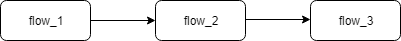
\includegraphics[scale=0.6,trim=0 0 0 0]{images/transformational-systems.png}
	\label{fig:transformational-systems}
\end{figure}

In contrast to that, reactive systems continuously interact with the environment. They constantly keep updating their state whenever some event is fired. Hence, state is essential in reactive systems.

\begin{figure}[!h]
	\centering
	\includegraphics[scale=0.6,trim=0 0 0 0]{images/reactive-systems.png}
	\label{fig:reactive-systems}
\end{figure}

\subsection {Challenges in Implementing Reactive Systems}
Implementing reactive systems is hard, because of continuous interaction between states and updates. With the help of following example, reactive systems can be explained in detail.

\begin{lstlisting}[language=JavaScript, caption=Sample example 1, label={lst:sample-example-1}]
var a = 1;
var b = 2;
var c = a + b;
b = 4;
console.log(c)
\end{lstlisting}
The output of the listing \ref{lst:sample-example-1} would be 3 because of the traditional programming approach. Change in the value of variable \textit{b} has no effect on variable \textit{c} because \textit{c} has been defined before. But in reactive systems, the line 2 is rather interpreted as a constraint instead of an assignment, so that the output would be 5. The value of variable c is always updated whenever value of \textit{a} or \textit{b} changes. 
To implement such reactive system, a manual approach would look similar to the following code:
\begin{lstlisting}[language=JavaScript, caption=Sample example 2, label={lst:sample-example-2}]
var a = 1;
var b = 2;
var c = a + b;
b = 5;
valueChanged();
console.log(c);


// This function will recalculates the value of c
function valueChanged(){
	c = a + b;
}
\end{lstlisting}
Above method naturally leads to following problems:

\begin{itemize}
	
	\item The function \textit{valueChanged} is scattered throughout the system. After each update of a or b, the triggering code should be inserted.
	\item There is a high chance that the developer may forget to insert the code and an important update can be missed.
	\item It is not possible to compose different reactions. One cannot express new constraints based on existing ones.
	\item There is no separation of concern.
	\item There is a lot of boilerplate code just to define a simple constraint. In the above example, just to express c = a + b, there is unnecessary code duplication which is less readable and less maintainable.
\end{itemize}
	
\section {Implementation of Reactive Systems}
Apart from the manual approach, there are multiple ways how the reactive system can be implemented. We will discuss the traditional approaches such as aspect-oriented programming, observer design pattern, promises and callbacks in this section. 
	
\subsection{The Observer Pattern}
The Observer Pattern(also known as Publish-Subscribe Pattern)\cite{understandingObserverPattern} is a way of reacting to changes. 
This pattern defines one-to-many relationships between objects such a way that when a state of one object changes, all dependent objects are updated automatically. 
It is suitable for any scenario, which requires push-based notification\cite{understandingObserverPattern}. 
As a refresher, a UML diagram is depicted in Figure~\ref{fig:observer-uml}. The drawbacks of the observer pattern are broadly discussed in literature  ``Deprecating the Observer Pattern'', which explains the problems in detail and concludes by proposing a built-in support for reactive programming abstractions as a solution\cite{deprecatingTheObserverPattern}. 
The pattern still suffers from nearly all aforementioned problems when using a manual approach. 
The only real advantage: through the observer pattern, a better modularity is achieved. 
The updated code is decoupled from the code that changes a value. 
This makes the code more readable and less error-prone. 

\begin{figure}[!h]
	\centering
	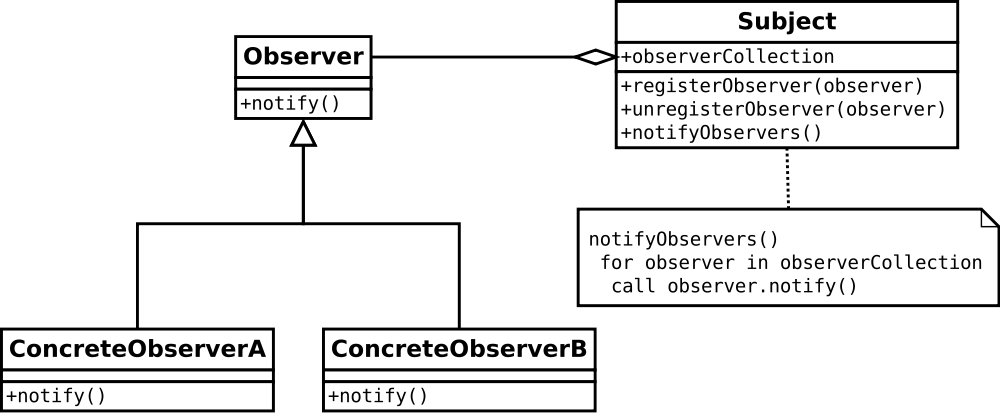
\includegraphics[scale=0.5,trim=0 0 0 0]{images/observer-uml.png}
	\caption{UML Class Diagram of the Observer Pattern}
	\label{fig:observer-uml}
\end{figure}

\subsection{Aspect-Oriented Programming (AOP)}
Aspect-Oriented Programming is a subset of Object-Oriented Programming. 
AOP aims at modularizing the CCC(cross-cutting concerns) throughout the application. 
These concerns are related to any code, which cannot be cleanly decomposed from rest of the application and leads to code duplication. 
With AOP, it is possible to define points in the code at which some update code should be executed. 
These so-called pointcuts are based on events such as call of a method, execution of exception handler. 
These events can be combined with logical operators to generate more complex pointcuts. 
To implement reactive systems, the code which is responsible for updating the states in the system could be implemented using AOP. There are several javascript libraries such as Dojo, JQuery AOP plugin, AspectJS that promise to address the CCC. 
However, AOP still has some drawbacks where dependencies have to be encoded manually.
\subsection{Callbacks}
For quite some time now, programmers have been simulating the management of events/notifications and corresponding responses with traditional programming techniques and asynchronous event handles like \textbf{callbacks}. 
Callbacks are nothing but javascript functions. 
These are called by any other function which accepts the first function as a parameter. 
Most of the time, a ``callback'' is a function that is called whenever an event happens. 
The difficult thing when trying to understand is the order in which the callbacks execute as the program runs. 
Nesting callbacks to achieve asynchronous tasks often leads to a problem called ``\textbf{callback hell}''\cite{callbackHell}. 
The only way to delay computation so that it runs after the asynchronous call return is to put the delayed code inside a callback function.
Callback hell problem can be handled to some extent by keeping the code shallow, modularizing the code and handling every single error. 

\subsection{Promises}
The problem imposed by callbacks can be dealt with \textbf{promises}. D. Wise and Daniel Friedman\cite{promiseKeyword} proposed the term promise as a proxy object that represents an unknown result that is yet to be computed. 
Libraries such as Q, JQuery, vow, have already implemented promises with some minor differences in syntax.
Furthermore, libraries like AngularJs\cite{angularjs}, MVC-based Javascript library for web applications and Dart, a class-based web programming language have provided the abstractions for implementation of promises. 
Promises provide the modularization of the code and easy to handle and understand. 
One problem of using \textbf{promises} is that once a \textbf{promise} is triggered, there is no way to stop it. 
Once fired, they will end and call callback method, either in a successful way or out in an error.


\section {Reactive Programming}
Developers have been using \textbf{procedural} and \textbf{imperative} programming from a long time. 
Object Oriented (OO) languages made programming more organized and structured, bringing in the concepts of inheritance and modularity. 
These programming paradigms consisted of a sequence of statements to be executed sequentially as encountered by the compiler to reach particular system state. 
Functional programming made the programming more declarative. 
In \textbf{functional programming}, the output of a program depends only on the input and refers to no external state, also has no side effects\cite{Gifford:1986:IFI:319838.319848}. 
Hence the program that takes a particular input always returns the same output irrespective of any other conditions.
Functional programs are designed to be reusable and composable. 
They also enforce immutability and functions can be composed of a chain to obtain the desired output. 
In functional programming, functions could be written more expressively also with a more intuitive handling of the current object with the \textit{this} keyword. 
The verbosity in a traditional way of defining functions is greatly reduced using lambda styled expressions.

Most of the modern systems are reactive and they respond to a specific event of interest by changing state. 
Designing, developing and debugging such systems is hard because most computations are triggered with asynchronous inputs which makes it difficult to trace the control flow back\cite{Margara:2014:WDD:2611286.2611290}. 
The birth of Reactive programming was to address the very same problem. A RP language provides abstractions with which a program is expressed as a series of reactions to observable events\cite{Bainomugisha:2013:SRP:2501654.2501666}. 
RP is based on the idea of ``Define, Watch \& React''\cite{RPvsFP} where the entities of interest are defined, those would be observed and the reactions are triggered based on the changes observed on the interested entities. 
In a non-RP setup, a value assignment to a data element is generally a ``snapshot assignment'' indicating that the value assigned would be based on a calculation at the time of assignment. 
Dependencies between data elements are never established. The values are read and assigned at particular assignment points in a program. 
RP aims to establish data dependencies between elements. 
Assuming a variable \textit{a} depends on variable \textit{b}, \textit{a} is assigned value based on the value of \textit{b} at a certain point of time in the program. 
If value of \textit{b} changes, this is propagated to reflect and update the value of \textit{a} accordingly. 
In simple terms, RP is modeled on the spreadsheet like model where cell dependencies are defined and an update on one cell triggers a series of dependent cells\cite{Bainomugisha:2013:SRP:2501654.2501666}.

RP handles an asynchronous sequence of data from the defined observable sequences. 
With the introduction of observer design pattern, observables could send multiple values over a period of time in response to a registration request from an observer. 
These values from the observable are asynchronous in nature and the observer has to handle them on a continuous basis over time. 
There are certain issues with the observer pattern that RP elegantly overcomes like the observer missing out on values that were sent from the observable before registration, the inversion of control with the observer pattern, the verbose non-declarative pattern of linking observables and observers etc. 
An author Stephen Blackheath, lists a few scenarios where designs based on observer pattern fail that RP overcomes \cite{whyFRP}. 
The article\cite{deprecatingTheObserverPattern} talks extensively about the shortcomings of the observer pattern. 
In traditional observer pattern, the programmer is expected to handle the logic around the registration of the observers and manage notifications; however, with RP, the programmer declaratively specifies the dependencies between the various observables and the reactions. 
The language runtime is expected to handle the propagation of values also reducing the errors and ensuring correctness. 
The study\cite{Salvaneschi:2014:ESP:2635868.2635895} makes a detailed empirical evaluation on the comprehensibility of RP in comparison to the traditional observer pattern in object-oriented programming. 
The study also highlights the reduction in side effects of callbacks and also the boilerplate code around the traditional observer pattern in object-oriented style when RP is used in place.

Scala.React\cite{deprecatingTheObserverPattern}, is library that implements composable reactive abstractions on Scala. Flapjax\cite{Meyerovich:2009:FPL:1639949.1640091} is Javascript framework for event-driven and reactive evaluation. These are Reactive languages that are based on the Functional programming style but do not integrate well with the mutable state of objects in the object-oriented style. These demand that, objects have to be recomputed from scratch in response to a change in a dependency. These are defined in a declarative way and updates on dependencies are handled by the runtime.

REScala\cite{Salvaneschi:2014:RBO:2577080.2577083} is a reactive language that bridges the gap between event-driven languages, functional reactive programming, and the object-oriented languages. The study\cite{Salvaneschi:2014:RBO:2577080.2577083} discusses the drawbacks of each of the above mentioned approaches applied in isolation and provides REScala as the solution that brings in the best of these into a single language. ReactiveX\cite{reactiveX} is a library that also brings in the declarative and functional programming into the OO world also providing event compositions with LINQ\cite{linq} styled operators, which we will look at in more details in the further sections.

Distributed REScala\cite{Drechsler:2014:DRU:2660193.2660240} brings reactive programming to distributed systems. Distributed software accounts to a huge chunk of software systems today and Distributed REScala brings in the reactive programming language support to distributed software across multiple hosts. The study\cite{Drechsler:2014:DRU:2660193.2660240} shows that existing algorithms for the update propagation in a single system are not suitable for a Distributed scenario and propose an algorithm (Source Identifier Update Propagation) for glitch-free propagation of dependency updates in distributed systems. The algorithm also makes no assumptions about the knowledge of a centralized topology of dependencies between values.

Distributed Reactive Middleware (DREAM) \cite{Margara:2014:WDD:2611286.2611290} is a middleware completely implemented in Java that focuses on consistency guarantees in a reactive distributed system. DREAM highlights the lack of research on the consistency guarantees of signal propagation between components in a distributed reactive scenario and proposes a middleware support that the components in a distributed reactive setup can utilize to define suitable properties and enforce the required consistency guarantees for the propagation of changes between the components.

We will look at ReactiveX, RxJS and BaconJS in detail in the next section as these are most commonly used reactive javascript libraries.

\subsection{ReactiveX}
ReactiveX is an API based on the idea of asynchronous programming based on events using observable streams. An author André Staltz, defines reactive programming as programming with asynchronous data streams\cite{introToRP}. ReactiveX is a programming API based on RP principles. It enables to programmatically express \cite{Doblander:2015:GEA:2675743.2776757} all the properties that are desired of Reactive systems\cite{reactiveManifesto}. In ReactiveX, various data types can be viewed as an observable that emits only a single data item. User input events can also be considered as observables that emit streams of data. The consumer deals with the incoming data when it is notified of the data from the stream.

In addition to this, there are range of operators that can be applied on the streams. A filter applied to a stream observes the stream and emits a new stream of values that satisfy the filter criteria. In ReactiveX, every stream is immutable and the operator observing a stream, emits a new stream of values, leaving the original unchanged. In essence, a key aspect of ReactiveX(RP in general) is the flexibility to compose \cite{Meyerovich:2009:FPL:1639949.1640091} asynchronous data into observable sequences.

ReactiveX facilitates notification of error and complete also in case of an error in an operation or when a stream is complete respectively by specifying functions in the observer to be notified of the corresponding events. The error and complete notifications, unlike the data notifications, are terminal and the association between the observable and the observer is ended. However, the error and complete functions are optional and an observer is free to leave them unimplemented. The observer can unsubscribe too from the observable to stop receiving notifications. Further, we will discuss RxJS, a Reactive Extension for javascript.

\subsection{RxJS}
RP has attracted more attention due to its ease of programming user interfaces\cite{Schuster:2016:RPR:2892664.2892666}\cite{Bainomugisha:2013:SRP:2501654.2501666}. The idea of ReactiveX has been employed for various platforms and programming languages and RxJS is javascript library that allows users the means to employ ReactiveX concepts into user interfaces. 

Asynchronicity and user-system interactivity \cite{Kristaly:2008:WTW:1389586.1389663} has been increasing consistently on the user interface of web applications especially with the introduction of Ajax technologies\cite{ajaxANewWayToWP} on the web pages. RxJS makes an attempt to take the user experience to the next level of responsiveness through event streams and event compositions. RxJS employs the ReactiveX practices along with the javascript's inherent query operators to build desired observables and have the observers notified of the events asynchronously.

\subsubsection{RxJS Concepts}
Asynchronous delivery of a value is readily available in vanilla javascript as of ES6\cite{ECMAScript} and callbacks have been used before promises. However, observables\cite{observable} facilitate delivering multiple values to subscribers asynchronously. Observables provide abstractions over a stream of events. Promises are synchronous executables with a single return value, whereas observables are asynchronous executables that return multiple values over time. 
\\
\textbf{Observables}
\\
Observables in ReactiveX can be conceptually viewed as the push equivalent of Iterables\cite{reactiveX}. The subscribers pull data from iterables, whereas the observers are notified of the availability of new information from observables through push mechanism, the \textit{next} method defined on the observers. With this idea, the subscribers are not locked in a synchronous request and there can be an infinite sequence of \textit{next} emissions from the observables to the observer.

Observables in ReactiveX also add another important idea of \textit{completed} and \textit{error} functions being defined at the observer, which are invoked by the observable on respective events. This lets the observer know that an observable has exhausted sending values, or an error has occurred when performing an operation on the observable. The calls to \textit{next} are generally referred to as emissions and the \textit{completed} and \textit{error} are called notifications. It is evident how elegantly errors are handled and pushed as normal data to the consumer. An error is not something that is dealt by the observable but is passed on to the subscriber along the pipeline and the subscriber is expected to handle the errors. There is no such explicit definition in the case of iterables.  

Observable is the basic building block of RxJS. The data produced by the producer is stored in observable which the consumer consumes. If the consumer is subscribed to the producer, it receives a signal from the observable whenever the data is pushed from the producer. Data available in the observable is not stored in the memory as opposed to an array which stores data in the memory. An observable represents event stream on which we can perform different methods as we can do on an array. For example, we can map the each value in an observable. There are two type of observables: Hot and Cold. According to an author Ben Lesh\footnote{\url{https://medium.com/@benlesh/hot-vs-cold-observables-f8094ed53339} , last accessed 23-08-2017}, if the underlying producer is created and activated during subscription, it is \textit{cold observable} and an observable is \textit{hot} if the underlying producer is either created or activated outside of its subscription.
\\
\textbf{Operators}
\\
RxJS is a combination of the best ideas from iterator pattern, observer pattern and functional programming\cite{reactiveX}. Before data is handed over to subscriber by an observable, there is a possibility that range of operators can be applied on the data streams. Each operator outputs an another observable without modifying the original data streams. This can be best understood with a representation using Marble diagrams. In the figure~\ref{fig:operator-marble-diagram},  a marble diagram is used to explain observables and transformation to another observable when an operator is applied. 

\begin{figure}[!h]
	\centering
	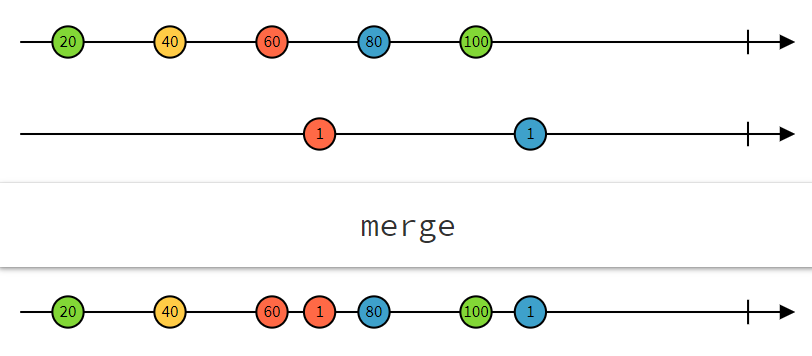
\includegraphics[scale=0.5,trim=0 0 0 0]{images/operator-marble-diagram.png}
	\caption{Marble diagram}
	\label{fig:operator-marble-diagram}
\end{figure}

Operators can be chained one of the other on observables to derive the desired results. Since the operators are chained, each operator is applied on the output of the previous operator and not on the original observable data streams. All the available operators in RxJS can be found in the online documentation\footnote{\url{http://reactivex.io/documentation/operators.html}}.
\\
\textbf{Subjects}
\\
Subjects can be both \textbf{observable} and an \textbf{observer}\cite{reactiveSubjects}. It is a special type of observable which allows values to be multicasted to many observers. Observables are unicast in nature. Subjects maintain the list of observers. Whenever different observers subscribe to the source observable is intercepted by the subjects and subjects multicast the data from source observable to the subscribed observers. When source publishes the value, the subject receives the value and it further broadcasts that value to the observer that are subscribed to the source observable. 


Subjects are implicitly used when an observable is shared between observers, which is the case when using \textit{hot observables}. When a \textit{share} function is called on an observable, a hot observable is implicitly created and subject acts as a proxy between the observable and the observers. The subjects handles the registration and disposal of subscriptions to the observable. The subject also acts as a single observer on the source observable. There are four types of Subjects: \textbf{AsyncSubject}, \textbf{BehaviorSubject}, \textbf{PublishSubject} and \textbf{ReplaySubject}.

\begin{figure}[!h]
	\centering
	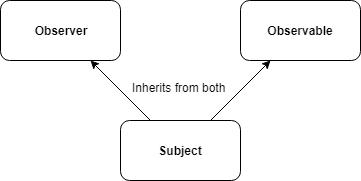
\includegraphics[scale=0.5,trim=0 0 0 0]{images/subjects.png}
	\caption{Subject}
	\label{fig:subject-diagram}
\end{figure}

\leavevmode
\\
\textbf{RxJS - Design}
\\
Understanding the internal workings of RxJS involves knowledge of design and functioning of the RxJS framework. RxJS code can be divided into four parts. The first part will define the creation of source observable. The second part, to derive the desired observable, we will apply some operators on the source observable. In the third part, we will subscribe to the source observable to receive the emitted values after the operators are applied. Lastly, we will unsubscribe from the source observable. Unsubscribing is an optional feature in RxJS as RxJS handles this by default but it makes sense to unsubscribe manually by a user if the source observable is emitting the values continuously and the user does not need values after a specific point of time. RxJS example code can be seen in a example listing~\ref{lst:rxjs-example}. As we discussed earlier, an observable is a collection of the data stream, we first need to create an observable. We can use functionality provided by RxJS to create an observable or we can create our own observable from scratch by wrapping any functionality that produces values over time. With the support of RxJS, we can convert multiple values, arrays, events into observables. 

\begin{lstlisting}[language=JavaScript, caption=RxJS example, label={lst:rxjs-example}]
/*
Increment value every 1s, emit numbers 0, 1, 2, ....
*/
const observable = Rx.Observable.create(function(observer) {
let value = 0;
const interval = setInterval(() => {
observer.next(value);
value++;
}, 1000);

return () => clearInterval(interval);
});

const evenNumbers = observable.map(function(x) {
// return the square of each value
return x * x;
}).filter(function(x) {
// filter the values which are even
return x % 2 === 0
}).take(3);

// variable subscribe is subscribing to evenNumbers observable
const subscribe = evenNumbers.subscribe(val => console.log(val));

//unsubscribe after 10 seconds
setTimeout(() => {
subscribe.unsubscribe();
}, 10000);

//Output to the console
0
4
16
\end{lstlisting}

In the example code, from line 4 to 12, variable \textit{observable} is defined as observable, which emits a sequence of numbers after 1000 milliseconds. In line 14 to 20, three operators are chained together and applied on the \textit{observable} to derived the desired observable \textit{evenNumbers}. Map operator is applied on \textit{observable} and returns the square of each emitted values. For example, \textit{observable} emits 0,1,2,3,4... and after \textbf{map} operator is applied, the new observable will emit the values 0,1,4,9,16.... The \textbf{filter} operator will then filter out the even values (0,4,16,36,64..) and pass on to the next operator. Lastly, the \textbf{take} operator will take only first 3 values(0,4,16) from the data stream. Thus, \textit{evenNumbers} observables holds the values 0,4,16. In the line 23, a subscriber \textit{subscribe} will subscribe to \textit{evenNumbers} observable and print the values emitted to the console. After 10000 milliseconds, we will unsubscribe to the \textit{evenNumbers} observable, which can be seen in the lines 26 to 28. After unsubscribing, the values emitted by \textit{evenNumbers} observable are discarded.


\subsection{BaconJS}
BaconJS is a functional reactive programming module for events in javascript which can transform event listener/handler to a functional event stream. BaconJS turns event streams into clean and declarative data streams by switching from imperative way to functional way. For example, replacing nested for-loops with functional programming concepts like map and filter. BaconJS emphasizes on working with event streams instead of individual events. \textbf{Eventstream} and \textbf{property} are the two kinds of observables in BaconJS. EventStream represents discrete values over the time. One can think of eventstreams as lists of events occurring over the time. For example, a promise that resolves after getting data from the API consists of events which can be modeled into event streams. The power of eventstreams is that they are composable. The tools to handle arrays for event streams are also be used on eventstreams such as filter events, map one event value to another. In the case of \textbf{properties}, they introduce the notion of continuous values which change over time. Any event streams can be easily converted to a property.  Properties are very much similar to \textbf{eventstreams} in behavior but properties may or may not have an initial value, properties are continuous whereas eventstreams are discrete. At any given point of time, an eventstream can be converted to property using inbuilt methods such as \textit{toProperty()}, \textit{scan()} and \textit{fold()}\cite{baconBlog}. 


\section{Debugging Software Programs}
Developing Software programs includes testing, updating and maintenance. Usually, every software contains bugs or errors, which are removed over the time. The errors can be coding errors, design errors, complex interactions and system failures. The process of removing the bugs by finding out the root cause is called Debugging. In debugging process, software programs are compiled and executed to identify and eliminate the bugs. The rise of IDEs(Integrated Development Environment) has reduced the syntax related errors to some extent but to its hard to detect logical errors in the program. To help the debugging process, developers use the debugger program. With the help of debuggers, users can step-through statements in a program by setting up breakpoints wherever necessary. When the program hits the breakpoint, the execution of the program is paused and a user can see the state of the program at that point in time. Debuggers also help user to see current execution stack which displays the stack history through which the control reached the specified breakpoint. Generally, debuggers are integrated with the development IDEs. Also, there are other independent debuggers such as \cite{oracleDebugger} and \cite{gnuDebugger} which run from command line and take a target program for analysis and inspection. In general, debuggers are developed for a particular programming language but there are debuggers such as GNU debugger\cite{gnuDebugger}, which can handle programs of multiple programming languages.

\subsection{Debugging Javascript}
Debugging is hard. But fortunately, modern browsers ship with a built-in javascript debugger. Javascript does not provide many debugging tools and, therefore it is challenging to debug any javascript program. In programming languages such as C++, Java, all objects are defined before the program is written and the user can use these definitions during the debugging process\cite{hoffman2000data}. Whereas, javascript is an interpretive language in which objects can be described dynamically. Javascript gives a user the power to assign new properties to objects as the program is executed. Such nature of javascript makes it hard to debug. There are different ways to debug javascript code such as using \textit{alert} statements, printing out values to console, using \textit{debugger} statement and using browser inbuilt debuggers. To understand the flow of the execution, a developer used to write alert or console.log statements which was extra code to the program. Using browser inbuilt debuggers, the developer can set breakpoints to a specific line in the program and examine the complete context of execution. After examining the values, the developer can resume the execution of the program. With the help of \textit{debugger;} statements, the user can achieve the similar functionality as setting up a breakpoint. 

\subsection{Debugging Reactive Programs}
Debugging reactive programs is a tedious task. In imperative programming paradigm, program execution can be tracked step-by-step with a breakpoint-based debugger; this is not possible with reactive programs. Assuming a reactive program can be tracked step-by-step, what should the debugger do when a value on which many other values depend is updated? Should it skip them? This would skip important steps. On another hand, moving from one update statement to another would also be quite confusing. Since some updates depend on other updates, countless values would have to be updated. Tracking all these updates with traditional debuggers is quite not possible.

In the article\cite{debugRxJS}, the author explains why debugging RxJS programs is hard with the help of traditional debuggers. The applications developed using reactive javascript libraries are more abstract than procedural code. In the article, author mentioned the ways RxJS application can be debugged. One has to rely on drawing a dependency graph or marble diagrams manually. An example of marble diagram is shown in the figure~\ref{fig:operator-marble-diagram}. It is not feasible to draw a dependency graph or marble diagram manually for large applications. So there is a need of new debugging tools to support debugging for reactive javascript libraries. In this thesis, we take a step forward to implement a google chrome extension to visualize and debug the application. We will discuss the tool in coming chapters.

\subsection{Jalangi Framework}
Jalangi framework\cite{Sen:2013:JSR:2491411.2491447} is a powerful    browser-independent(dynamic) analysis framework for javaScript. The framework helps the user understand few useful abstractions and an API that simplifies implementation of dynamic analyses for javascript. The framework is independent of browser and an operating system. The framework instruments the javascript code and allows a user to further implement various dynamic analysis techniques. When the framework instruments the code, it creates hooks in the output and those hooks are monitored whenever there is an operation such as read or write to variable, function calls etc.


Working of Jalangi framework is illustrated in the figure~\ref{fig:jalangi-components}. First, the framework reads the javascript code and performs instrumentation of the code and outputs instrumented code. Then, the instrumented code can be run in the browser or Node.js environment. We will not discuss how we can use an instrumented code in the Node.js environment as it is out of the scope for this thesis. With the help of API provided by the framework, the user can invoke callback functions. By invoking the callback functions, the user can intercept the execution of events and perform further analysis if required. 

\begin{figure}[!h]
	\centering
	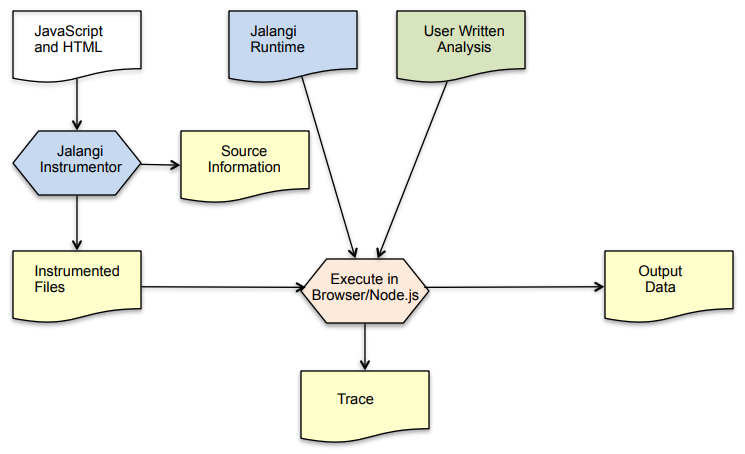
\includegraphics[scale=0.5,trim=0 0 0 0]{images/jalangi-components.png}
	\caption{Jalangi framework components}
	\label{fig:jalangi-components}
\end{figure}

\section{Google Chrome Developer Tools}
The Chrome Developer Tools(DevTools) are a group of debugging and web authoring tools build into Google Chrome\cite{devtools}. The DevTools provide an interface where web developers get deep access into the internals of the browser and their web application. To access the DevTools, open a web page in Google chrome and use keyboard shortcuts \textit{Ctrl+Shift+I(Windows)} and \textit{Cmd+Opt+I(Mac)}. By right-clicking on a web page and selecting an option \textit{Inspect} also opens up DevTools. By default, DevTools ships with panels such as Elements, Console, Sources, Network etc.

\begin{figure}[!h]
	\centering
	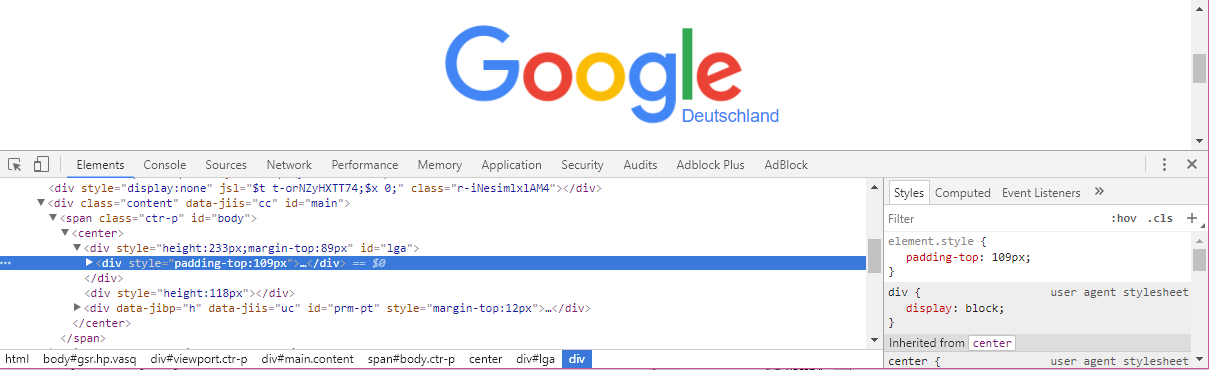
\includegraphics[scale=0.5,trim=0 0 0 0]{images/chrome-devtools.png}
	\caption{Chrome Developer Tools}
	\label{fig:devtools}
\end{figure}

In figure~\ref{fig:devtools}, we can see how DevTools looks when opened. The Elements tab window is split into two panels with HTML on the left and CSS, javascript debugging on the right. HTML panel gives the overview of Document Object Model(DOM) of the page. Developer can modify the HTML or CSS code and the effect can be seen on the page. The console tab shows all the information logged into the console by the running javascript code. The logged values can be either warning messages or error messages or the information logged by the user in the code. This tab is extensively used by web developers to debug the javascript code. Sources tab provides an overview of all the files related the current web page. The user can set breakpoints in the javascript files for the debugging purpose. The Network tabs provide a detailed information regarding various HTTP calls made by the browser. 

\subsection{Extending Chrome Developer Tools} \label{section:extending_devtools}
DevTools can be extended to add additional features. 
A DevTools extension is any functionality that is added in the form of an extension to enhance the debugging capabilities. 
An extension can be embedded as a new tab or a sidebar in the Elements tab. 
The extension is structured very similar to any other Chrome extensions\cite{devtoolsextension}. 
With the help of the extension, a developer can interact with the current web page, get access to debugger etc. 
DevTools provides user a large pool of javascript APIs\cite{devtools}. 
The elements of the manifest file are listed in \cite{devtoolsmanifestfile}. 
The manifest file(manifest.json) tells Chrome, information about the extension such as name, permissions, version etc. 
The file declared as \textit{devtools\_page} in the manifest file has access to DevTools API, \textbf{chrome.devtools}. 
The Background page is created when an extension is loaded and it handles the user events and corresponding views for the events. 
Architecture of chrome DevTools extension is depicted in the figure~\ref{fig:extension-architecture}. 
Components communicate with each other by message passing.

\begin{figure}[!h]
	\centering
	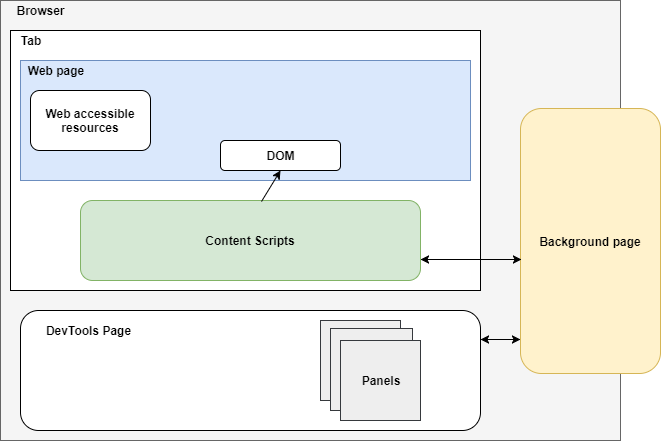
\includegraphics[scale=0.7,trim=0 0 0 0]{images/chrome-extension-architecture.png}
	\caption{Chrome Extension Architecture}
	\label{fig:extension-architecture}
\end{figure}

Content scripts in chrome extension are the list of javascript files which run in the context of web pages when the page is loaded\cite{contentscripts}. They have the ability to modify the current web page since they have access to the DOM. But they do not have the ability to modify the loaded javascript code for the current page. There are two ways to inject content scripts: inject statically for all the pages or programmatically. In programmatically injection method, the \textit{devtools\_page} requests the background page to inject the content script. A message is sent to background page with the content script file names to load. The background page then handles the injection using \textbf{chrome.tabs.executeScript} API. In the statically injection method, the list of all the content scripts files to be injected are mentioned in the manifest file. In the manifest file, the developer can also specify other information like the time of injection whether before injecting all the scripts or after. Here, the background page acts as a bridge between content scripts of the page and devtools\_page of the extension.

Content scripts are executed in a special environment which is often referred to as an isolated world\cite{contentscripts}. Javascript defined in the inspected page and content scripts do not have any knowledge of each other. They both run in isolation and handle their respective events on their own\cite{contentscripts}. According to google chrome developers documents, chrome prevents direct access between content script and inspected pages\textquotesingle javascript file due to security reasons. Although content script has no knowledge about the web page\textquotesingle s javascript, it can still access the DOM of the page. The communication between inspected page and the content script can only happen through message passing API window.postMessage\cite{contentscripts}. With the help of API call, specific event listeners defined in the content script and the inspected page can communicate with each other.


\section{Related Work}
As we discussed earlier, it is difficult to debug reactive programs. Due to the limitations of traditional javascript debuggers, there emerged a need of new debuggers. Some of them we will discuss in this section. The blog\cite{debugrxjsblog} suggests users to use the \textbf{do} operator for debugging the code. The \textbf{do} operator does not modify data in the observable but helps the user to log the subsequent values to the console. The operator can be used as shown in the below example.
\begin{lstlisting}[language=JavaScript, caption=Do operator usage, label={lst:do-operator-example}]
var shortLowerCaseName$ = name$
.map(function (name) {
return name.toLowerCase(); })
.do(console.log);
\end{lstlisting}

In the above example, \textbf{do} operator in the line no. 4 will log all the values which are passed from \textit{map} operator after converting values to lowercase. The issue with the \textbf{do} operator is, it is an overhead code which should be removed in the production environment. 

\leavevmode
\\
\textbf{RxVision}
\\
While learning RxJS, an author Jared Forsyth developed an open source tool RxVision\cite{rxvision}. The tool helps the user to understand the flow of the data stream by visualizing the streams in real time. The author also provides the user an online playground where users can write RxJS code and the tool will visualize it instantly\cite{rxvisionplayground}. Unfortunately, this tool is not under active development and it does not support latest RxJs version. The tool not only visualizes the code but also provide an information such as source code line number. It is hard to understand the visualization since it does not give much information regarding variable names and map them to the visualization. 
\leavevmode
\\
\textbf{RxFiddle}
\\
This is another tool developed to debug Reactive Extensions by Herman Banken as a part of Master thesis\cite{rxfiddle}.  
This tool is similar to RxVision but supports both RxJS version 4 and 5. The tool visualizes the data flow through observable in more detailed manner. 
Currently, it supports RxJS code snippets and lacks the support for input streams\cite{rxfiddle}. This tool can be used in both browser and Node environment.  

